% !TeX root =thesis.tex

\chapter{Introduction}
%Superfluidity in many-body fermionic system is one of the most dramatic and fascinating topic in physics. It calls the attention and effort from generation of physicists.  The study is dominated with one particular fermions, electrons.  However, this system suffers from one difficulty as the interaction  in a particular system is usually fixed and cannot be tuned experimentally.  
From  a methodological view, a physical system  would be very desirable for developing and  verifying a theory  if  it can be described with  as few parameters as possible,  and each parameter is as tunable as possible. One such system is the ultracold dilute fermionic alkali gas with the Feshbach resonance.  Dilute fermionic alkali gas was cooled into degenerate region in 1999 \cite{DeMarco1999}. Not long after that,  superfluidity was observed for such systems in 2003 \cite{Regal2003}.  In dilute ultracold fermionic alkali gas, it is sufficient in many phenomena to describe an atom-atom interaction with one single parameter, namely the s-wave scattering length, $a_{s}$, because the gas is very dilute and experiments are performed at very low temperatures.       

The other desirable property is the ability to  tune the effective interaction strength, i.e., in the present case, the s-wave scattering length, $a_{s}$ through  Feshbach resonances.  One atomic energy level  splits into several hyperfine levels under a magnetic field,  due to the hyperfine interaction between nuclear spins and electronic spins. Hyperfine spin indices provide a good set of quantum numbers for a single atom.  In the theory of  atom-atom interactions, a channel refers to a specific configuration of hyperfine spin indices of one atom pair. Different channels usually  have different magnetic moments and therefore have different Zeeman energies in the presence of a magnetic field.  The difference of the Zeeman energies can then be tuned by changing the magnetic field.  In addition, a channel is no longer an exact eigenstate when the atom-atom interaction is taken into consideration because the interaction is mostly due to the overlap between electronic parts of  the two-atoms' wave-functions. As a result, channels are hybridized.  The effective potential of each channel is also different.  The potential of one  channel  may be deep enough to sustain a bound state.  This channel is then called \emph{``closed-channel''}.  For a certain magnetic field,  the energy level of this bound state might be close to the zero-energy threshold of the other channel, usually called \emph{open-channel}, and two channels  thus strongly hybridized.  The low-energy scattering properties in the open-channel is then dramatically modified.   In such a situation, two atoms approaching each other in the open-channel may ``spend a certain amount of time in the closed-channel'' and then reemerge in the open-channel.  Atoms in the open-channel seem to feel an enhanced effective interaction.  This phenomenon is known as Feshbach resonances.    We will present a  quantitative analysis about alkali gas in Chpater \ref{sec:intro:one} and  Feshbach resonances in two-body context in Chapter \ref{sec:intro:twobody}. 




A very desirable property of the Feshbach resonance is that the effective interaction is tunable experimentally through the Zeeman energy difference between channels which is in turn  tunable through  instruments such as a magnetic field.  
This unique ability gives physicists a rare opportunity to study  a many-body system under various interaction strengths,  and thus connect different physics originally developed separately.  Particularly for the fermionic gas, there are a series of  theoretical works about uniform treatment of  BEC and BCS since the 1960s \cite{Eagle,LeggettCrossover,Nozieres,RanderiaBEC}, for which dilute ultracold fermionic alkali gas with  Feshbach resonances provides the perfect testing grounds.  Indeed,  these theories works quite well  qualitatively.  

%One important characteristic quantity of Feshbach resonance is $\delta_{C}$N (see detail in Chapter \ref{sec:intro:twobody} for details): when detuning from resonance is smaller than it, open-channel atoms dominate and closed-channel can be neglected.  The effective interaction can still be characterized by $a_{s}$.  One seems to acquire a ``magic knob'' that can tune the interaction between atoms.  On the other hand, when negative tuning is much larger than $\delta_{C}$, atoms in closed-channel have comparable weight to that of open-channel or even dominate them.  Two channels need to be considered at the same time.  


%This thesis tries to look into the idiosyncrasy of the Feshbach resonance in contrast with a true ``Simple'' knob of the interaction strength.
\begin{figure}[htbp]
\begin{center}
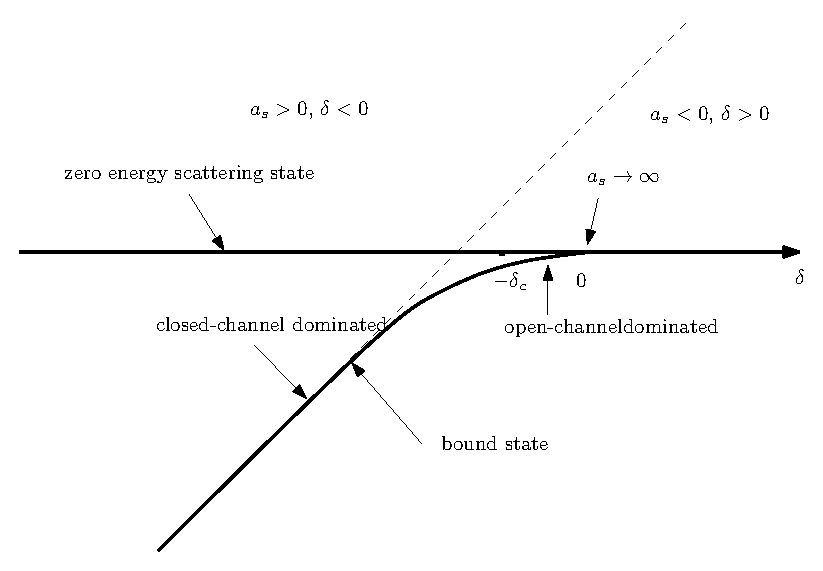
\includegraphics[width=0.8\textwidth]{levels}
\caption{Energy levels in a Feshbach resonance\label{fig:intro:levels}} 
\parbox{0.7\textwidth}{\small $\delta$ is the energy detuning from the resonance point, where the resonant point is defined as the point where the open-channel effective s-wave scattering length diverges, $a_s\to\pm\infty$.  The horizontal line stands for the zero energy s-wave scattering state, $\psi\sim\nth{r}-\nth{a_s}$, which exists for any detuning.  The lower line stands for the real bound state, which only exists for negative detuning ($\delta<0$, $a_s>0$). The dash line stands for the (uncoupled) closed-channel bound state.  An interesting point to notice is that the real bound state appears earlier than the cross point of the (uncoupled) closed-channel bound state level and zero energy. Another important point to notice is the negative detuning $-\delta_c$.  When the negative detuning is smaller than $\delta_c$, this real bound state is composed mostly with atoms in the open-channel and vice verse.  See Chapter \ref{sec:intro:twobody} for details about $\mathcal{K}$ and $\delta_c$.   }

\end{center}
\end{figure}

  The two-body theory of the Feshbach resonance has a characteristic  parameter, $\delta_c$, defined as  the detuning energy at which the weight of the bound state shifts from predominated in the open-channel to predominated in the closed-channel (see Fig. \ref{fig:intro:levels}).  Na\"{i}vely speaking, in the negative detuning side of any resonance (i.e. $\delta<0$), particles should mostly stay  in a (virtual) bound-state of the closed-channel (or ``virtual state'' in some other resonances).  However, at the resonance point  of the Feshbach resonance ($a_s\to\pm\infty$), atoms are mostly still in the open-channel, and they do so down to a negative detuning $\delta\sim-\delta_c$. Only when the detuning from resonance is much far away than $\delta_c$, do atoms have the majority weight in the closed-channel.    
  
  When considering a many-body problem, an important question is how this energy scale, $\delta_c$, compares to a typical many-body energy scale, namely, the Fermi energy of the free fermionic atoms. In the region not too far away from resonance ($\abs{\delta}\ll\delta_{c}$), the closed-channel weight is negligible if the Fermi energy is much smaller than $\delta_c$, (i.e., \emph{broad resonance}).  Crossover experiments are usually performed at detuning not too far from the resonance, and hence the closed-channel can be safely ignored at the many-body level. Eventually, when the detuning is too far away, $\abs{\delta}\gg\delta_{c}$, the bound state is almost like the    uncoupled closed-channel bound state with a little dressing from the open-channel.  We nevertheless do not concern such cases for the broad resonance because crossover phenomena have already be well covered in both BEC and BCS ends with $\abs{\delta}\ll\delta_{c}$. The problem can be well-described as a two-species fermion system with a tunable interaction.  The Feshbach resonance indeed serves as a simple ``magic'' knob to change the interaction strength.  The original  theories developed on  single-channel models  apply to this case directly.  This is also the situation for two  popular experiment cases (${}^{6}\text{Li}$ atoms at 834G, $^{40}\text{K}$ atoms at 224G).   Many theoretical works have been developed using the single-channel model as these original works or using the tow-channel model within the broad resonance assumption (e.g. \cite{Holland01,HoUniversal,Fuchs04}). On the contrary, when the Fermi energy of the free fermionic atoms is  comparable to or even larger than $\delta_c$, the closed-channel has to be included at the many-body level even for small detuning. Such a situation, previously considered in some works \cite{GurarieNarrow}, is the focus of the current thesis. 
  
  Nevertheless, one crucial simplification comes from  the fact  that relevant uncoupled closed-channel bound state is  tightly bound, with spatial extension much smaller than  many-body scales, e.g. the interparticle distance, (but often larger than the potential range).  This fact enable us to treat the Pauli exclusion between two channels perturbatively. It is not necessary to handle all the  fermion species simultaneously, which probably requires quite different techniques  other than those discussed in this thesis. 

To complicate the problem even further,  real experimental configurations often have one common hyperfine species between the two channels. There are three hyperfine species in the  two channels instead of four species (two for each channel).  Two most common setups (${}^{6}\text{Li}$ at 834G, $^{40}\text{K}$ at 224G) both contain three species of fermions although they are the broad resonance.  The Pauli exclusion principle prevents  atoms of both channels from occupying the same level simultaneously because of this common species.  The inter-channel Pauli exclusion has no counterpart in two-body physics. This peculiar effect  in many-body crossover problems has  received little theoretical attention up to now.    Nevertheless,   narrow resonances do exist \cite{ChinRMP} and it is not  inconceivable to perform many-body experiments using such resonances.  The central concern of this thesis is about these situations. 

Roughly speaking, turning from two-body systems to many-body systems brings three effects into the original two-body problem.  The first effect is closely associated with the Fermi energy:  For a many-body fermionic system at low temperature, most fermions are inactive; only the fermions close to the Fermi surface participate in the interaction processes. Therefore, energy often needs to be measured from the Fermi surface instead of from zero as in a two-body situation. This aspect has been extensively studied previously \cite{GurarieNarrow}.

The second effect is about counting. Unlike in the single-channel problem, there are two relevant densities in the two-channel problem: the density of atoms in the open-channel, $n_{o}$, and the density of atoms in the closed-channel, $n_{c}$. When the closed-channel weight is small (broad resonance), it is all right to treat the total density as the same as the open-channel density.  However, in the narrow resonance, where the closed-channel weight is not negligible, counting becomes complicated.  Extra care is required to specify which channel the  quantities, such as ``density'', belong to.  This aspect has been  also extensively studied previously \cite{GurarieNarrow}.

The last effect is unique for the three-species problem, where one common species is shared by both channels.  The phase spaces of two channels are overlapped because of the Pauli exclusion caused by the common species. This effect is controlled by the wave-function overlapping of states in the two channels. A rough estimate of this overlapping can be made: The uncoupled closed-channel bound-state which is in resonance with the open-channel zero energy threshold has  relatively small  spatial extension, $a_c$.  Its binding energy $E_b$ is close to the Zeeman energy difference between two channels, $\eta$.  On the other hand, fermions in the open-channel fill the lowest  momentum states up to typically the Fermi energy, $E_F$.  By a simple dimensional argument, the ratio $E_F/\eta$ must control the overlapping effect. This effect has  not been addressed in any theoretical work to this author's knowledge.  How it modifies the many-body picture is the central topic of this thesis. 

We can see this from a slightly alternative aspect using two-fermion molecule gas for the uncoupled closed-channel bound state. We assume that the molecule size is $a_{c}$ and the total number of molecules is $N$.  Assuming further that the bound-state is close to threshold,   the bound-state wave function can then be written as $A/(k^{2}+\kappa^{2})$, where $\hbar^{2}\kappa^{2}/2m=E_{b}$, (see Appendix \ref{sec:pathInt2:short-range}). The prefactor ``$A$'' can be determined  by normalization, $\sum_{k=0}^{1/a_{c}}\abs{\psi}^{2}\sim{}N$. Now  we consider all atoms in a typical many-body scale, e.g. the Fermi energy, $E_{F}$, which is going to overlap with levels occupied in the open-channel. Usually, the Fermi energy is much smaller than the energy scale of the closed-channel bound state, $E_{F}\ll{}E_b$.  The total number of atoms in $[0,E_F]$ is roughly $N\cdot(k_{F}a_{c})^{3}$, which is much smaller than $N$. This means that in the two-channel problem, the low momenta,  ($k\lesssim{}k_F$), are still dominated by the open-channel component even when the total number of atoms in the closed-channel is comparable or higher than the total number  of atoms in the open-channel because atoms in the closed-channel are mostly in  high-momentum states.     

The present thesis is divided as follows:
Chapter \ref{sec:intro:one} to  \ref{sec:intro:1channel} review several important concepts used in the thesis.  Chapters \ref{ch:path2} and \ref{ch:excitation} then present my main work  and Appendix \ref{ch:mean}  lists an earlier attempt using a roughly equivalent but less-flexible approach.  

More specifically, Chapter \ref{sec:intro:one} briefly reviews  dilute ultracold alkali gas.   Section \ref{sec:intro:as} in particular examines the idea of ``universality'', which is one of the central ideas in our treatment of the two-channel model.  Chapter \ref{sec:intro:twobody} goes over the Feshbach resonance in two-body physics and  the concept of  the narrow (broad) resonance is introduced. Chapter \ref{sec:intro:1channel} reviews the single-channel BEC-BCS crossover problem as well as the path-integral approach solving it. This chapter serves as the starting point for the solution of the two-channel model. After these reviews,   Chapter \ref{ch:path2} and Chapter \ref{ch:excitation} present my work on the three-species narrow Feshbach resonance within a many-body path-integral framework, in detail.   Chapter \ref{ch:path2} discusses the mean field result while Chapter \ref{ch:excitation} discusses fermionic and bosonic excitations. An earlier attempt   based on the BCS ansatz  approach in mean-field level is given in Appendix \ref{ch:mean}.  Chapter \ref{ch:conclusion} discusses our procedures and their conclusions.  

\chapter{Dilute ultracold alkali gas}\label{sec:intro:one}
  Since the 1990s, dilute  alkali gas has been cooled into quantum degenerate region where the thermal de Broglie wavelength ($\frac{h}{\sqrt{2\pi{m}k_{B}{T}}}$) is comparable or larger than the interparticle distance.  Not long after successfully cooling the bosonic atoms, fermionic alkali gas was also available in the degenerate region.  Because of the ultra-low temperature (in the order of nK), and the extreme diluteness ($10^{12}\sim10^{15}\text{cm}^{-3}$), the atoms are mostly \emph{free} except when they are  close.   This particular property simplifies theoretical analyses tremendously (see Sec. \ref{sec:intro:as} for details).  In this chapter, we review a few aspects of the dilute ultracold alkali gas that are closely related to the current thesis.     

\section{A single atom and its hyperfine levels}
In experiments on ultracold alkali gas, a magnetic field ($\mathbf{B}$) is the most common physical quantity to manipulate.   Let us first study an   isolated atom in the presence of a magnetic field.  An alkali atom has only one electron in its outer shell.  All the rest electrons are in the filled inner shells which  has no total magnetic moment.  So we only need to consider the spin of the outermost electron,  $\mathbf{S}$, for interaction with the magnetic field. In addition, a magnetic field also interacts with the atom's nuclear spin, $\mathbf{I}$.  The full spin-part Hamiltonian is
\begin{equation}
\begin{split}\label{eq:intro:1atom}
H_{spin}&=A \mathbf{I}\cdot\mathbf{S}-\mu_{e}\mathbf{B}\cdot\mathbf{S}-{\mu}_{n}\mathbf{B}\cdot\mathbf{I}\\
&=A \mathbf{I}\cdot\mathbf{S}-\mu_{e}{B}{S_{z}}-{\mu}_{n}{B}{I_{z}}
\end{split}
\end{equation}
The first term with a characteristic energy $A$ describes the hyperfine interaction, while the next two terms describe Zeeman energies of the outer electron and nuclei respectively. $\mu_{e}$ is the electronic magnetic moment, while $\mu_n$ is the nuclear magnetic moment.  In the second line, we take the direction of the magnetic field as the z-direction. This Hamiltonian can be diagonalized by introducing the total spin 
\begin{equation}
\mathbf{F}=\mathbf{S}+\mathbf{I}
\end{equation}
When the magnetic field is zero, the two Zeeman energy terms in the above Hamiltonian vanish.  Thus, $(F,F_{z})$ are good quantum numbers and all states with the same $F$ are degenerate.   When the magnetic field is finite, $(F,F_{z})$ cannot diagonalize the Zeeman energy terms, and therefore are no longer good quantum numbers. Nevertheless, we can still label the atomic  states with these two numbers via the adiabatic connection to the levels in the zero magnetic field.  For a finite magnetic field, except for states with the highest and lowest $F_{z}$, namely, $\pm{}F$, each other state is a mixture of different $(S_{z}, I_{z})$ or $(F,F_z)$.  Fortunately, $S$ is just equal to $1/2$ for an alkali atom. So each state is mixed with at most  two sets of quantum numbers $(S_{z}, I_{z})$. At high magnetic fields, the first hyperfine coupling term in Eq. \eqref{eq:intro:1atom} is dominated by the last two terms of Zeeman energies and the eigenstates are approximately described by the quantum numbers $(S_{z},I_{z})$.  (See Fig. \ref{fig:intro:li6}.)

\begin{figure}[htbp]
\begin{center}
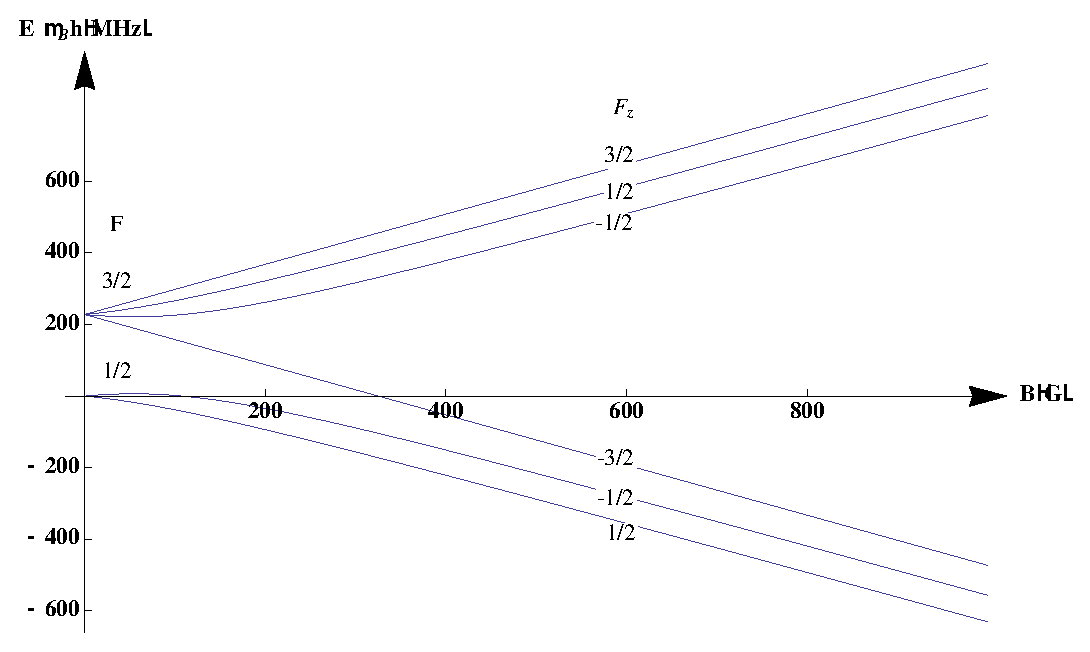
\includegraphics[width=0.8\textwidth]{hyperfineLi6}
\caption{Hyperfine structure of a single \textsuperscript{6}Li atom } 
Levels are marked with $F$ and $F_{z}$ {(see Footnote \ref{foot:intro:f} in page \pageref{foot:intro:f})} %Note that the energy of the $\ket{F=\nth{2},F_z=-\nth{2}}$ state first increases with the magnetic field, $B$, at low field then decrease at high field. In the same way, the energy of the $\ket{F=\frac{3}{2},F_z=-\nth{2}}$ state first decreases and then increases with the magnetic field.  
\label{fig:intro:li6}
\end{center}
\end{figure}



\section{Two-body interactions}
Things would be very boring if there was only the single-atom Hamiltonian.  Before discussing the interaction itself, let us introduce one important concept related to it.    The term ``channel'' is used to refer one  configuration of hyperfine spins for one atom pair in interaction, $\ket{F^{(1)},F_{z}^{(1)}}\otimes\ket{F^{(2)},F_{z}^{(2)}}$ . \footnote{Remember that $(F,F_{z})$ are only labels; they do not stand for the total angular momentum unless there is no magnetic field.\label{foot:intro:f}}    Channels are good basis for non-interaction pairs.  A pair of atoms in one channel would stay in this channel  forever in the absence of  interactions between atoms.  Considering the present case of alkali atoms, two alkali atoms mostly interact  through the overlapping of their electron wave-functions in the dilute limit.  Thus, besides the atom-atom distance, the interaction is mostly a function of electronic spins, with negligible dependence on nuclear spins.  Schematically the interaction can be written as 
\begin{equation}\label{eq:intro:two}
V=f(r)+g(r)\mathbf{S_{1}}\cdot\mathbf{S_{2}}
\end{equation}
Here the spatial part of the interaction is coupled with electronic spins. The hyperfine levels that diagonalize the single atom Hamiltonian are no longer eigenstates for this interaction.  In another word, the interaction has non-diagonal terms between channels and therefore hybridizes them. Instead, states with definite electronic spins form a good approximate basis for the atom-atom interaction.  Nonetheless, most experiments are performed in the so-called high-field region,  where the Zeeman energy terms dominate the hyperfine interaction term in the single-atom Hamiltonian (Eq. \ref{eq:intro:1atom}).   Recalling that one hyperfine state is at most mixture of the two $(S_{z}, I_{z})$ states.  In the high-field, one of them always dominate the other; therefore               the electronic spin $S_z$ is approximately a good quantum number for a hyperfine level, and the original hyperfine levels (channels) serve as a good starting point as the zeroth order approximation.  When the hybridization is taken into account, multichannel scatterings are possible.  The most interesting thing in these multi-channel scatterings is the possibility of a resonance.  One of them is the so-called Feshbach resonance:  The potential in one channel may be deep enough to sustain a bound-state. This channel is named ``closed-channel''. When this bound-state energy is close to the zero-energy threshold of another channel, named ``open-channel'', the low-energy scattering properties in the open-channel are dramatically modified.  This resonance turns out to be extremely useful in   cold atom experiments.  Chapter \ref{sec:intro:twobody} reviews its theory for  a two-body system. The more involving many-body problem is then the central theme of this thesis and is discussed in Chapter \ref{ch:path2} and \ref{ch:excitation} in detail. 

Let us illustrate above discussion in  one example.  In a common experimental setup for $^{6}$Li (Fig. \ref{fig:intro:li6}), experiments are usually  prepared with atoms in the two lowest hyperfine levels: described by the  direct product of two states, $\ket{F=\nth{2},F_{z}=-\nth{2}}\otimes\ket{F=\nth{2},F_{z}=+\nth{2}}$.  This is a good approximation until the two atoms are very close.  Recalling that the atom-atom interaction (Eq. \ref{eq:intro:two}) conserves the z-component of the total angular momentum, $F_{z}^{(1)}+F_{z}^{(2)}$, this channel mixes with four other possible channels of the same total z-direction angular momentum, i.e. $F_{z}^{(1)}+F_{z}^{(2)}=0$: $\ket{\nth{2},-\nth{2}}\otimes\ket{\frac{3}{2},+\nth{2}}$, $\ket{\frac{3}{2},-\nth{2}}\otimes\ket{\nth{2},+\nth{2}}$, $\ket{\frac{3}{2},+\frac{3}{2}}\otimes\ket{\frac{3}{2},-\frac{3}{2}}$, $\ket{\frac{3}{2},+\frac{1}{2}}\otimes\ket{\frac{3}{2},-\frac{1}{2}}$ (All states are labeled as $\ket{F,F_{z}}$).  Various resonances can take place.  Note that close to the resonance, it is normally sufficient to consider only the  channel that is in resonance, while neglect all other channels.  Another important aspect is whether the two channels share one single hyperfine species or not.  In the former case,  totally three hyperfine species are involved while in the later case, four hyperfine species are involved.   The closed channel in the most studied resonance with a magnetic filed close 834G, is approximately $\ket{\frac{3}{2},-\nth{2}}\otimes\ket{\nth{2},+\nth{2}}$ and the resonance is a three-species resonance\cite{ZhangThesis,ChinRMP}. 

\section{Universality,  Bethe-Peierls boundary conditions, the s-wave scattering length, and  two-body density matrices \label{sec:intro:as}}
One important aspect of the interaction in dilute ultracold alkali gas is that for many purposes, it is sufficient to characterize the interaction  by a single two-body parameter, namely, the s-wave scattering length, $a_s$,  because  both the density  and the temperature, are very  low. This is often interpreted as we can replace the real potential with a pseudo potential, $U(\vr)=\frac{4\pi{}a_{s}\hbar^{2}}{m}\delta(\vr)$\cite{pethick, LeggettBEC}.  Nevertheless, an alternative interpretation of $a_s$ \cite{LeggettBEC, Tan2008-1,Tan2008-2,CombescotTan} is more useful in this work.  For a short-range potential, where the potential range, $r_c$, is much smaller than the average interparticle distance, $a_0$,  particles are free-like  in the majority of the time.  They only interact  when two particles are close to each other.  We can thus schematically divide the space into two domains: $\mathcal{D}$, where any two particles are more than $r_c$ away from each other; and otherwise, $\mathcal{I}$. Most physical quantities would be very easy to calculate if only considering the free part, $\mathcal{D}$.  In a low-energy (ultracold) dilute system, we only need to consider  pair-wise interaction while neglect all the three-body or more-body interactions.  In addition,  $\mathcal{D}$ takes the majority of the space due to the same reason.     The effect of the potential on wave-function in the short-range region, $\mathcal{I}$, can be taken simply as   a boundary condition on the wave-function in the free part $\mathcal{D}$, $\psi(r)\xrightarrow{r\to0}\psi_{0}(r)$.  For an isometric $\psi_{0}(r)$, the lowest order in the radial coordinate $r$ is $\nth{r}$. \footnote{The extra $\nth{r}$ factor is there for  radial wave function in 3D.}  Including the next order, a constant,  we have $\psi_{0}(r)\propto\nth{r}-\nth{a_s}$ barring the normalization.  All these consideration gives us the simplest non-trivial boundary condition on  a wave function
\begin{equation}\label{eq:intro:Bethe}
\psi(r)\xrightarrow{r\to0}A\br{\nth{r}-\nth{a_s}}
\end{equation}
which is also known as the Bethe-Peierls boundary condition\cite{BethePeierls}.    $a_{s}$ is fully determined by two-body physics.  This simple boundary condition applies to two-body, few-body, as well as many-body systems, and has been proved to be a very powerful tool in solving various problems.  

Eq. \ref{eq:intro:Bethe} coincides the zero-energy s-wave scattering wave function, which explains the name of parameter ``$a_s$'', the s-wave scattering length. Nevertheless,    we did not mention anything about zero energy so far, although $a_{s}$ is defined for zero energy in the scattering theory context.  In fact,  this boundary condition (Eq. \ref{eq:intro:Bethe}) applies generally to  any low (positive or negative) energy solutions as long as the energy involved is much lower than the energy scale in the interaction domain $\mathcal{I}$.  Hence, this boundary condition applys  to close-to-threshold bound states as well.  The s-wave wave function of a weak bound-state reads $\psi(r)=\nth{r}e^{-r/a_s}$ in $\mathcal{D}$, which matches the Bethe-Peierls boundary condition with a positive $a_{s}$ for  $r\ll{}a_{s}$. The exponential decay factor of the wave function, $a_{s}$, is directly related to the binding energy, $E_{b}$, with the often cited relation.
\begin{equation}
 E_{b}=\frac{\hbar^{2}}{2m_{r}a_{s}^{2}}
\end{equation}
Here $m_{r}$ is the reduced mass for center of mass, which is equal to half of the atom mass for a pair of the same atoms.  This immediately clears one often confusing and counter-intuitive fact, that a positive  $a_s$ is associated to a bound state.  In the standard scattering theory, a positive $a_s$  is usually associated with a repulsive interaction, which obviously does not support a bound state.\footnote{This seeming paradox can be resolved carefully within scattering theory as follows. In the scattering theory, only when the interaction is weak, and phase shift as well as $a_s$ are small, we have the fact that a repulsive interaction leads to a positive phase shift and a positive $a_s$; while an attractive interaction leads to a negative phase shift and a negative $a_s$.  No simple relationship of signs holds for a strong interaction, where a bound state might form.  In fact, the phase shift changes as much as $2\pi$ when a bound state starts to form; therefore, $a_s$ is large and  changes sign over the threshold. }

  Eq. \ref{eq:intro:Bethe}, does not fix the normalization on the wave function. This normalization factor, encapsulating effects from particles outside the immediate interacting pair, appears in many physical quantities.  In a dilute and low-energy system,  its square is proportional to the so-called \emph{integrated contact intensity}, $C$, introduced by Tan \cite{ Tan2008-1,Tan2008-2,CombescotTan}.  For the limit $r_c\to0$, the integrated contact intensity, $C$, and the s-wave scattering length, $a_s$, are sufficient to describe several important physical quantities, such as  internal energy.  A particular useful one for this thesis is the limit at high-momentum of the particle number distribution of particles, 
 \begin{equation}
 \lim_{k\to\infty}n_k=\frac{C}{k^4}
 \end{equation}
 Note that here \emph{high-momentum} does not mean the absolutely high-momentum, it means lower than the characteristic momentum of potential $1/r_c$, but higher than any other scale, $1/a_0$,...  
 Indeed, when the short-range approximation and low-energy approximation apply, we expect that the two-body correlation at  high-momentum ($\gg{k_{F}}$) does not change much from a two-body system to a many-body system.  In this high-momentum region, we can always use   the two-body wave function as good approximation. 
 
 In many-body physics, various physical observable quantities are related to one set of  quantities, namely, density matrices,  $\av{\Psi^\dg(x_{1})\cdots\Psi^\dg(x_{N})\Psi(x'_{N})\cdots\Psi(x'_{1})}$. In fermionic system,  the one-body density matrix ($N=1$) for an interacting system is often very close to the one for the free particles, although the difference can be important for some theories, such as Landau Fermi liquid theory.  A two-body density matrix ($N=2$) is often  used because it is often different from the two-body density matrices of the free fermions qualitatively, such as in the case of BCS pairing. Formally, we can decompose a two-body density matrix into an orthogonal basis
 \begin{equation}\label{eq:intro:2bodyDM}
 \av{\Psi^\dg(x_1)\Psi^\dg(x_2)\Psi(y_2)\Psi(y_1)}=\sum_nC_n\phi_n^\dg(x_1,x_2)\phi_n(y_1,y_2)
 \end{equation}     
 When one or a few $C_n$ are macroscopic,  some special quantum phenomena often emerges.  Especially when only one parameter, $C_{0}$, is macroscopic, the system can often be interpreted as one macroscopic wave function, $\phi_{0}(x_{1},x_{2})$, (which is often called  order parameters).\cite{Leggett}  This can serve as a starting point for several phenomena, such as  BCS superconducting,...
 
Zhang and Leggett developed independently another universality theory based on two-body density matrices \linebreak[2] \cite{shizhongUniv}, which actually take a more general form of boundary conditions than the Bethe-Peierls boundary condition with $a_{s}$.   They asserted that for a short-range potential and a low temperature, as in the case of  dilute ultracold alkali gas, the basis wave functions $\phi_n$  in Eq. \eqref{eq:intro:2bodyDM} follows the two-body wave function at short-range. This is actually similar to Eq. \eqref{eq:intro:Bethe}.  Instead of requiring the simplest form of $\psi_0$ given in Eq. \eqref{eq:intro:Bethe}, they require a more general wave-function that solves the  Hamiltonian at two-body level.  Not surprisingly, many physical properties are determined by the normalization factors  as using the Bethe-Peierls boundary condition.  

In this thesis, similar idea is used.  We assume that the closed-channel correlations follow the its two-body bound-state wave-function at high energy (i.e. short-range).   An open-channel correlation follows its two-body  wave-function at short-range, but its intermediate range does not do so because of the sensitive nature of resonance.   The current thesis focus on how this wave-function are modified. 
 
 
 \chapter{The  Feshbach resonance in two-body physics\label{sec:intro:twobody}}
 As discussed in Sec. \ref{sec:intro:as}, a two-particle interaction in a dilute system is often approximated by a pseudo-potential characterized with a s-wave scattering length $a_{s}$.   The drastic  change  of $a_{s}$  obtained by tuning the energy difference  between two channels  through a magnetic field in the Feshbach resonance gives  experimentalists a rare ability to tune the interaction strength between two atoms.  And this possibility is extremely useful to study BEC-BCS crossover where the interaction varies from weak to strong.  
 
Here we briefly review the Feshbach resonance in a two-body system.   As discussed in Chapter \ref{sec:intro:one}, a hyperfine level is an eigenstate for an isolated single atom.  However, when two atoms interact, most of the interaction comes from  electrons with only negligible effects from nucleons .  As a result, hyperfine levels are no longer true eigenstates of the two-body system.  Nevertheless, hyperfine levels can serve as  good approximated quantum numbers and we are going to call a pair of hyperfine indices a ``channel''.  Different channels in general have different  interactions.  They are decoupled at the lowest order.  In a magnetic field, different channels differ in energy at threshold, where two atoms are infinitely away from each other, due to the Zeeman energy which is mostly determined by the electronic magnetic moment because  the electronic magnetic moment is much larger than the nuclear magnetic moment.  This energy difference is easy to tune through a magnetic field.  

When the mixing between channels are taken into consideration, the simple single-channel scattering becomes the multi-channel scattering.  Especially, when the one channel's threshold is close to a bound-state in the other channel, the low-energy scattering property of that channel is dramatically altered.  Its phase shift  changes $2\pi$;  its s-wave scattering length $a_{s}$ blows to infinity and then jumps to the infinity of the opposite sign.  This is essentially what happens in a Feshbach resonance, studied by Fano\cite{Fano} and Feshbach \cite{nuclear} for nuclear and atomic physics in 1960s.  Here we  mostly follow the treatment by Leggett \cite{Leggett} (with some different symbols to comply with the rest of this thesis). 
\footnote{In order to be consistent  with  other parts of the thesis, we here use some different symbols comparing to the original works by Leggett \cite{Leggett}.  Here we list them, with the symbols from \cite{Leggett} in parenthesis.  $U$ ($=-V$): open-channel interaction; $V$ ($=-V_{c}$): closed-channel interaction; $Y$ (=-$g\cdot{}f$): inter-channel coupling; $E_{b}$ ($=\epsilon_{0}$): binding energy of the closed-channel bound state; $r_{c}$ ($=r_{0}$): potential range; $\eta$ ($=\epsilon_0+\tilde\delta$): the Zeeman energy difference between two channels; $\mathcal{K}$ ($=\kappa$) see its definition in Eq.\ref{eq:intro:kappa}.}

The  Hamiltonian for  the coupled open- and  closed- channel can be written as a $2\times2$ matrix 
\begin{equation}\label{eq:intro:ham}
\hat{H}(r)=
\begin{pmatrix}
-\frac{\hbar^{2}}{2m_{r}}\nabla^{2}-U(r)&\;&-Y(r)\\
-Y(r)&\;&-\frac{\hbar^{2}}{2m_{r}}\nabla^{2}+\eta-V(r)
\end{pmatrix}
\end{equation}
where the  zero energy is taken as the energy of two atoms in the open-channel with infinite separation. $\eta$ is the  difference in the Zeeman energies of the two channels.  The first column (row) stands for the open-channel and the second column (row) stands for the closed-channel.  All the interactions are short-range.  For a s-wave solution, we have the radial part as 
\begin{equation}
\psi(r)=\nth{r}\mtrx{\chi(r)\\\chi_{c}(r)}
\end{equation}
The coupled time-independent \sch equations in the radial direction read as:
\begin{align}
-\frac{\hbar^{2}}{2m_{r}}\chi''-U\chi-Y\chi_c&=E\chi\label{eq:intro:open}\\
-\frac{\hbar^{2}}{2m_{r}}\chi_c''+\eta\chi_c-V\chi_c-Y\chi&=E\chi_c\label{eq:intro:close}
\end{align}

We now expand the closed-channel component $\chi_{c}$ over the eigenstates of the isolated closed-channel Hamiltonian, $\chi_{c}=\sum_{i}c_{i}\phi_{i}$, where $\phi_{i}$ satisfies \sch equation of the isolated closed-channel
\begin{equation}\label{eq:intro:sch2}
-\frac{\hbar^{2}}{2m_{r}}\phi_{i}''-V \phi_{i}=-E_{b}^{(i)}\phi_{i}
\end{equation}
We denote $\phi_{0}$  the wave function  in resonance and $c_{0}$ its coefficient.  Here we assume that the energy differences between eigenstates, $\phi_{i}$'s, are larger than any other energy scales in the problem.  This guarantees $c_{0}$ dominates any other $c_{i}$'s.  So, $\chi_{c}\approx{}c_{0}\phi_{0}$.  Na\"{i}vely speaking, the resonance is expected to happen at the point where the closed-channel bound state has its energy exactly at the threshold of the open-channel.  This leads us to introduce the relative detuning, $\tilde\delta=\eta-E_{b}$. By comparing Eq. \ref{eq:intro:open} and Eq. \ref{eq:intro:sch2}, it is easy to show 
\begin{equation}\label{eq:intro:closeCoeff}
\chi_{c}=\frac{\phi_{0}}{E-\tilde\delta}\int{dr'}\,\phi_{0}^{*}(r')Y(r')\chi\br{r'}
\end{equation}
provided that  $\phi_{0}$ is normalized (for radial component).  Inserting the expression of $\chi_{c}$ into the \sch equation of the open-channel component $\chi$, Eq. \ref{eq:intro:open}, we get 
\begin{equation}\label{eq:intro:chi}
-\frac{\hbar^{2}}{2m_{r}}\chi''-(U+E)\chi+\frac{1}{E-\tilde\delta}\int_{0}^{\infty}K(r\,r')\chi(r')dr'=0
\end{equation}
where the kernel $K(r\,r')$ is
\begin{equation}\label{eq:intro:Krr}
K(r\,r')\equiv\phi_{0}(r)\phi_{0}(r')Y(r')Y(r)
\end{equation}
The  \sch equation of the  decoupled open-channel is
\begin{equation}\label{eq:intro:chi0}
-\frac{\hbar^{2}}{2m_{r}}\chi''-(U+E)\chi_{0}=0
\end{equation}
Note that $\chi_{0}(r)\overset{r\to0}\rightarrow0$ and $\chi_{0}(r)\overset{r\to\infty}\rightarrow{A}(1-r/a_{bg})\label{eq:intro:abg}$ , where $a_{bg}$ is the background s-wave scattering length of the isolated open-channel.\footnote{Note that we are dealing with the internal wave function $\chi_{0}$ here, i.e. the wave-function in the region $\mathcal{I}$, instead of the external wave function as in Sec. \ref{sec:intro:as}; therefore, the boundary condition for $r\rightarrow0$ in Sec. \ref{sec:intro:as} actually corresponds the boundary condition $r\rightarrow\infty$ here.}  Multiply Eq. \ref{eq:intro:chi} by $\chi_{0}$ and Eq. \ref{eq:intro:chi0} by $\chi$, integrate from $r=0$ to a  distance $r_{0}$ much larger than the potential range, $r_{c}$, subtract them, we find,
\begin{equation*}
\int_{0}^{r_{0}}dr\mbr{\chi_{0}(r)\chi''(r)-\chi_{0}''(r)\chi(r)}+\frac{2m_{r}E}{\hbar^{2}}\int_{0}^{r_{0}}dr\chi_{0}(r)\chi(r)
=\frac{2m_{r}/\hbar^{2}}{E-\tilde\delta}\int_{0}^{r_{0}}dr\int_{0}^{r_{0}}dr'\chi_{0}(r)K(rr')\chi(r')
\end{equation*}
Using the Green's theorem on the first integral, we find 
\begin{equation}
\chi_{0}(r_{0})\chi'(r_{0})-\chi_{0}'(r_{0})\chi(r_{0})+\frac{2m_{r}E}{\hbar^{2}}\int_{0}^{r_{c}}dr\chi_{0}(r)\chi(r)
=\frac{2m_{r}/\hbar^{2}}{E-\tilde\delta}\int_{0}^{r_{0}}dr\int_{0}^{r_{0}}dr'\chi_{0}(r)K(rr')\chi(r')
\end{equation}
Here we can use the boundary condition by $\chi_{0}(r)\overset{r\to\infty}\rightarrow{A}(1-r/a_{bg})$, $\chi(r)\overset{r\to\infty}\rightarrow\tilde{A}(1-r/a_{s})$.  $Y(r)$ is a short-range interaction and thus $K(r,r')$ only picks the short-range parts of $\chi(r)$ and $\chi_{0}(r)$, which varies little for different detuning. Consequently,  the R.H.S approaches a constant.  For the scattering solution at  $E=0$, the last terml on the L.H.S. is zero, and we have 
\begin{equation}
\nth{a_{s}}-\nth{a_{bg}}=\frac{2m_{r}/\hbar^{2}}{\tilde\delta}\int_{0}^{\infty}dr\int_{0}^{\infty}dr'\chi_{0}(r)K(rr')\chi(r')
\end{equation}
Contrary to the previous guess, $a_{s}$ does not diverge at the point $\tilde\delta=0$ because of the original interaction in the open-channel, $a_{bg}$.  We can introduce a quantity $\mathcal{K}$, the detuning where $a_{s}$ diverges, through the implicit equation ($\mathcal{K}$ shows up in R.H.S as well)
\begin{equation}\label{eq:intro:kappa}
\mathcal{K}\equiv-\frac{2m_{r}a_{bg}}{\hbar^{2}}\int_{0}^{\infty}{dr}\int_{0}^{\infty}dr'\chi_{0}(r)K(rr')\chi_{\tilde\delta=\mathcal{K}}(r')
\end{equation}
And if we define the ``real detuning'' $\delta\equiv\tilde\delta-\mathcal{K}$, which is the detuning from the real resonant point, where $a_{s}\to\pm\infty$, we have 
\begin{equation}\label{eq:intro:asK}
a_{s}(\delta)=a_{bg}\br{1+\frac{\mathcal{K}}{\delta}}
\end{equation}
This is consistent with the empirical formula of the Feshbach resonance
\begin{equation}
a_{s}(B)=a_{bg}\br{1+\frac{\Delta{B}}{B-B_{0}}}
\end{equation}
where $B_{0}$ is the magnetic field at which the $a_{s}$ diverges, i.e., the  resonant point.  Comparing the above two equations, we see that $\Delta{B}=\mathcal{K}(\partial\delta/\partial{B})^{-1}$.  %Here $\partial\delta/\partial{B}$ is the magnetic momentum difference between two channels.  
\begin{figure}[htbp]
\begin{center}
\includegraphics[width=0.8\textwidth]{FeshbachAs}
\caption{S-wave scattering length in Feshbach resonance} 
\label{fig:intro:Feshbach}
{\small The dashed line is $y=a_{bg}$.}
\end{center}
\end{figure}

Let us now consider the bound state,\footnote{We wish to stress again the difference between a uncoupled closed-channel bound-state $\phi_{i}$ and a real bound state  formed by atoms from both open- and closed-channel.   The closed-channel bound state, $\phi_{i}$, is the eigenstate of the  isolated closed-channel Hamiltonian.  It is not a real eigenstate for the full two-channel Hamiltonian.  On the other hand, the full  Hamiltonian has bound eigenstates (i.e. $E<0$) at large negative detuning (in the two-body context).  The bound state solution for a two-channel eigenstate has components in both the open-channel and the closed-channel.  The open-channel weight is often larger when close to the resonance; consequently, such bound-states are often called open-channel bound-states.  Only at large negative detuning, the real two-channel bound state, mostly composed of close-channel component, coincides with the close-channel bound-state, $\phi_{i}$ to a large degree.}
where $E<0$.  We define
\begin{equation}\label{eq:intro:ab}
a_{b}(E)\equiv\frac{\hbar}{(2m_{r}\abs{E})^{1/2}}
\end{equation}
 Here, we only study the bound state close to threshold with a binding energy much smaller than the binding energy of the uncoupled closed-channel bound state, $\phi_{0}$, namely, $\abs{E}\ll{}E_{b}$.  Therefore, we have  $a_{b}\gg{a_{c}}$.  Outside the range of potential $r_{c}$,  the wave function is proportional to $e^{-r/a_{b}}$. For $r_{c}\ll{}r\ll{}a_{b}$, this wave-function can be expanded as  $1-\frac{r}{a_{b}}$, just as the Bethe-Peierls boundary condition (or the s-wave scattering wave function) we discussed in Chapter \ref{sec:intro:as}.  Note that $a_{b}(E)$ is not identified as $a_{s}$ a priori.  Through a  procedure similar as previous,  it is not hard to find
\begin{equation}
\frac{a_{bg}}{a_{b}}-1=\frac{-\mathcal{K}}{\delta+\mathcal{K}-E}
\end{equation}
We have assumed the short-range part of the bound-state wave function $\chi$ does not change much from the short-range part of the scattering state \footnote{This is guaranteed by the boundary condition of $\chi(r)\to1-r/a_{s}$, which fixes the normalization of the short-range part of the wave function ($\chi{r\to0}$) to be the same, namely $1$. As a result, all the integral term over the short-range kernel $\iint{drdr'}K(r,r')\chi_{0}(r)\chi(r')$  give the similar value as  $\mathcal{K}$ at the resonant point, Eq. \ref{eq:intro:kappa}.};  therefore $\mathcal{K}$ stays like a constant.  Provided both $\delta$ and $\abs{E}$ are much smaller than $\mathcal{K}$, this yields\begin{equation}\label{eq:intro:abKE}
a_{b}=a_{bg}\frac{\mathcal{K}}{\delta-E}
\end{equation}
It is not hard to see that $a_{b}$ indeed  coincides with the s-wave scattering length $a_{s}$ in Eq. \ref{eq:intro:asK} when $\abs{E}\ll\abs{\delta}$. Thus we will use $a_{b}$ and $a_{s}$ interchangeably hereafter. This is actually an example of our discussion about the Bethe-Peierls boundary condition in Chapter \ref{sec:intro:as}. Using the concept of the Bethe-Peierls boundary condition, we do not need to distinguish the zero energy scattering state and the negative energy bound state, and we can arrive the same conclusion easily.  

  Using Eqs. \ref{eq:intro:ab} and \ref{eq:intro:abKE}, it is easy to obtain an equation for $E$
\begin{equation}
(\abs{E}+\delta)^{2}-2\delta_{c}\abs{E}=0 
\end{equation}
where $\delta_{c}$ is defined as 
\begin{equation}\label{eq:intro:deltaC}
\delta_{c}\equiv\frac{\mathcal{K}^{2}}{\hbar^{2}/m_{r}a_{bg}^{2}}
\end{equation}
And the solution for the negative detuning, i.e. $\delta<0$, is
\begin{equation}\label{eq:intro:bindE}
\abs{E}=\delta_{c}-\delta-\sqrt{\delta_{c}^{2}-2\delta\delta_{c}}
\end{equation}
We can also calculate the ``relative weight'' on probability of the closed-channel for a normalized open-channel component, $\chi_{n}$, of the wave function ($\int{}\chi_{n}(r)^{2}dr=1). $\footnote{Note here the normalization on $\chi(r)$ is different from the most cases of this section, where $\chi(r)$ is normalized by  requiring $\chi{}\overset{r\rightarrow\infty}\rightarrow{}(1-r/a_{b})\text{ or }e^{-r/a_{b}} $ here. The difference is an extra $(a_{b})^{-1/2}$ for the wave function and that contributes the extra factor $a_{b}^{-1}$ in Eq. \ref{eq:intro:lambda}.} 
\begin{equation}
\label{eq:intro:closeWeight}
\lambda=\br{\frac{1}{E-\tilde\delta}}^{2}\abs{\int{}dr'\phi_{0}(r')Y(r')\chi_{n}(r')}^{2}
\end{equation}
Comparing this with Eq. \ref{eq:intro:kappa}, and assuming the short-range part of $\chi_{n}(r)$ does not differ from $\chi_{o}(r)$ much except the normalization, we  find 
\begin{equation}\label{eq:intro:lambda}
\lambda=\nth{(E-\tilde\delta)^{2}}\frac{\hbar^{2}}{2m_{r}a_{bg}}\frac{\mathcal{K}}{a_{b}}
\end{equation}
For $\abs{\delta}\lesssim\delta_{c}\ll\mathcal{K}$,  we have 
\begin{equation}\label{eq:intro:shiftK}
E-\tilde\delta\approx\mathcal{K}
\end{equation}
We can simplify $\lambda$ further
\begin{equation}\label{eq:intro:lambda}
\lambda\approx\frac{\hbar^{2}}{2m_{r}a_{bg}}\nth{(\mathcal{K}a_{b})}=\br{\frac{\abs{E}}{2\delta_{c}}}^{1/2}
\end{equation}
This shows that  $\delta_{c}$ is a ``characteristic'' energy scale. When $\abs{\delta}\gg\delta_{c}$, Eq. \ref{eq:intro:bindE} gives $E\approx\delta$ , and the above equation gives $\lambda=\sqrt{|\delta|/(2\delta_{c})}\gg1$: this simply means that when the negative detuning is large, weight is predominently in the closed-channel; the real mixed bound state is a closed-channel bound state ($\phi_{0}$) slightly dressed with the open-channel component; therefore the binding energy is very close to the binding energy  of the uncoupled closed-channel bound state, $\phi_{0}$.  The often quoted relation between $a_{s}$ and the binding energy, Eq. \ref{eq:intro:ab},  is not valid here.  On the contrary, when $\abs{\delta}\ll\delta_{c}$, Eq. \ref{eq:intro:bindE}  gives $\abs{E}\approx\delta^{2}/\delta_{c}\ll\abs{\delta}$,  and Eq. \ref{eq:intro:lambda} then gives $\lambda\approx{\delta/(\sqrt{2}\delta_{c})}\ll1$.  Here, the closed-channel weight is much smaller than that of the open-channel; the real bound-state is essentially an open-channel affair with little dress-up from the closed-channel.  Eq. \ref{eq:intro:ab} is valid in this case. % It is not hard to  estimate $\delta_{c}$. 

When dealing with  many-body problems, another important energy scale comes into play, namely, the Fermi energy, $E_{F}$.  When $E_{F}$ is much smaller than $\delta_{c}$, i.e. a \emph{broad resonance},  the closed-channel has only negligible weight close to resonance, which is the situation of interest. In such a case, it is a good approximation to take the Feshbach resonance as only a knob to tweak the interaction in the open-channel.  On the contrary, when $E_{F}$ is close or even larger than $\delta_{c}$, i.e. a \emph{narrow resonance}, the closed-channel weight can be  significant clsoe to  resonance; as a result, it is necessary to explicitly take the closed-channel into account in the many-body framework.  

One important remark about the above discussion is that whether a resonance is ``broad'' or ``narrow'' is a many-body concept and is relative.  For one particular resonance with a fixed $\delta_{c}$, in a infinite dilute system (i.e. a two-body system) with a zero Fermi energy,  $E_{F}=0\ll\delta_{c}$, it is a broad resonance.  As the system becomes denser and denser, $E_{F}$ increases and the resonance becomes less and less broad; finally, when $E_{F}$ is in the order or even larger than $\delta_{c}$, the resonance becomes a narrow one.  In the real experimental system of the ultracold alkali gases, the achievable density has a certain range, so does the Fermi energy range, $E_{F}$; therefore the ``broadness'' or ``narrowness'' of a resonance is not as flexible. 










\chapter{The single-channel BEC-BCS crossover\label{sec:intro:1channel}}
In this chapter, we briefly review the BEC-BCS crossover in a single channel.   The idea to describe the BEC and BCS on the same footing stems back several decades \cite{Eagle, LeggettCrossover, Nozieres, RanderiaBEC}.  %One way to interpret BCS is through the existing macroscopic eigenvalue of two-body density matrix (see Sec. \ref{sec:intro:as})\cite{Leggett}.   This eigenvalue corresponds the more familiar anomalous expectation, $\av{a_{\uparrow-\vk}a_{\downarrow\vk}}$.  If simply taking it as wave function of a two-fermion molecule, this eigenfucntion, $\ket{\psi}=(\sum_{\vk}c_{\vk}a^{\dg}_{\uparrow\vk}a^{\dg}_{\downarrow-\vk})\ket{0}$ is very large in size (coherent length), much larger than the average particle distance.  Therefore overlap between different ``molecules'' is significant.   
The BCS theory can be understood as the following: fermions form  ``giant molecules'' and those molecules then condense simultaneously.    It is not hard to show that the  BCS ansatz is equivalent to  the  coherent state of a two-body pair $\psi^{\dg}=\sum_{\vk}c_{\vk}a^{\dg}_{\uparrow\vk}a^{\dg}_{\downarrow-\vk}$
\begin{equation}\label{eq:intro:BCScoherent}
\prod_{\vk}(u_{\vk}+v_{\vk}a^{\dg}_{\uparrow\vk}a^{\dg}_{\downarrow-\vk})\ket{0}=A\exp{}(\sum_{\vk}c_{\vk}a^{\dg}_{\uparrow\vk}a^{\dg}_{\downarrow-\vk})\ket{0}
\end{equation}
where $c_{\vk}=( v_{\vk}/u_{\vk})$. The size of these ``giant molecules'' is  much larger than the interparticle distance.
Moving away from the BCS end toward the BEC end, pairs shrink as the interparticle attraction becomes stronger.  On the BEC side, two-fermion molecules are smaller than the interparticle distance and therefore a well-defined object. However, the binding energy now is much larger than the typical many-body energy scale and condensation does not happen at the same time when molecules form.  Nevertheless,  at low enough temperature, we can still consider the formation of molecules and their condensation  at the same time, compatible with the  the same framework used for BCS.  

In the single-channel BEC-BCS crossover model, one imagines a ``magic'' knob that can tune the interaction strength along the crossover.  The many-body fermion  system sweeps from  BCS of a fermionic atom system to BEC of diatomic molecules  in response to the increase of attraction.   This directly applies to the broad-resonance of the two-channel case as well, where the closed-channel weight is negligible and only serves  to modify the effective interaction strength in the open-channel.  We mostly follow the path-integral treatment by Randeria and the company \cite{RanderiaBEC, Randeria1997, Randeria2008}.
%\subsection{Path integral for one channels}
% !TeX root =thesis.tex
%\subsection{Path integral approach for single channel\label{sec:pathInt}}
\label{sec:pathInt}
They have studied this problem with a path integral approach which is proved to be a  nice tool for the problem due to its flexibility and readiness to be   extended for the higher order fluctuations.  In the next two chapters, this method will be adapted  further for the two-channel model. 

We start with an attractive $\delta$-potential in the coordinate space.  This potential is not equivalent to the  reduced pairing potential used in the original BCS work.  The reduced pairing potential only couples  particles of the opposite momentum and does not support simple form of Hubbard-Stratonovich transformation, which is essential to solve the problem in the path integral formulation. 

  The Hamiltonian with the chemical potential of the system can be written as   
\begin{equation}
\hat{H}-\mu\hat{N}=\sum_{\sigma}\int{d^{d}\vr}c^{\dagger}_{\sigma}(\vr)\br{-\nth{2m}\nabla^{2}-\mu}c^{}_{\sigma}(\vr)-g\int{d^{d}\vr}c^{\dagger}_{\uparrow}(\vr)c^{\dagger}_{\downarrow}(\vr)c^{}_{\downarrow}(\vr)c^{}_{\uparrow}(\vr)
\end{equation}
Introducing the quantum partition function $\mathcal{Z}=\int{\bigD(\bar\psi,\psi)\exp\br{-S[\bar\psi,\psi]}}$, where $\bigD(\bar\psi,\psi)$ denotes the functional integral over all possible wave function $\psi$ and $\bar\psi$, and the action $S[\bar\psi,\psi]$ can be written down from the Hamiltonian
\begin{equation}\label{eq:pathInt2:actionPsi}
S[\bar\psi,\psi]=\int^{\beta}_{0}d\tau\int{d^{d}\vr}\mbr{\sum_{\sigma}\bar\psi_{\sigma}(\vr,\tau)\br{\partial_{\tau}-\nth{2m}\nabla^{2}-\mu}\psi_{\sigma}(\vr,\tau)-g\bar\psi_{\uparrow}(\vr,\tau)\bar\psi_{\downarrow}(\vr,\tau)\psi^{}_{\downarrow}(\vr,\tau)\psi^{}_{\uparrow}(\vr,\tau)}
\end{equation}
The fermion fields $\psi_{\sigma}$ and $\bar\psi_{\sigma}$ being two independent Grassmann variables, notice that  they are not complex conjugate to each other as in the usual operator language because  complex conjugate is not a well-defined concept for Grassmann variables. 

This system can be solved with Hubbard-Stratonovich transformation.   Introduce an auxiliary field (functional variable) $\Delta(\vr,\tau)$ coupled with a pair $\psi_{\uparrow}(\vr,\tau)\psi_{\downarrow}(\vr,\tau)$. %Here we follow the normal notation from path integral, $r$ is four tempo-space coordinator.  
We write down first the Gaussian integral of $\Delta$
\begin{equation}
1=\int{\bigD(\bar\Delta,\Delta)}\exp\br{-\nth{g}\int{d\tau{d}^{d}r}\bar\Delta\Delta}
\end{equation}
Note that we absorb the extra constant of integration into the measure of $\bigD(\bar\Delta,\Delta)$.
And with a shift of $\Delta(\vr,\tau)\rightarrow\Delta(\vr,\tau)-g\psi_{\uparrow}(\vr,\tau)\psi_{\downarrow}(\vr,\tau))$, we have 
\footnote{$\int{\bigD(\bar\Delta,\Delta)}\cdot1$ is only a constant factor on partition function $\mathcal{Z}$ and has no effect on real physical quantity; therefore, we can take it as 1. (This is equivalent to  divide the $\mathcal{Z}$ by a constant)}
\begin{equation}\label{eq:pathInt:expHS}
\exp\br{g\int{d\tau{}d^{d}r}\bar{\psi}_{\uparrow}\bar\psi_{\downarrow}\psi_{\downarrow}\psi_{\uparrow}}=
\int{\bigD(\bar\Delta,\Delta)}\exp\bbr{-\int{d\tau{d^{d}r}}\mbr{\nth{g}{\bar\Delta}{\Delta}-\br{\bar\Delta\psi_{\downarrow}\psi_{\uparrow}+\Delta\bar\psi_{\uparrow}\bar\psi_{\downarrow}}}}
\end{equation}
Note that  $\Delta(\vr,\tau)$ (or $\bar\Delta(\vr,\tau)$) comes from  Grassmann fields $\psi(\vr,\tau)$ (or $\bar\psi(\vr,\tau)$). Therefore, they are not related to each other as complex conjugate either.  Nevertheless, at the mean field level or only at the phase fluctuation around the mean field values, $\Delta$  and $\bar\Delta$ are indeed complex conjugate.  Consequently, we will just take $\Delta$  as normal bosonic field in the following and often simply treat $\bar\Delta$ as $\Delta$'s complex conjugate in the following. Now the interaction term can be replaced.
\begin{align*}
\mathcal{Z}=&\int{}\bigD(\bar\psi,\psi)\int{\bigD(\bar\Delta,\Delta)}\\
&\;\exp\bbr{-\int{d\tau{d^{d}r}}\mbr{\sum_{\sigma}\bar\psi_{\sigma}\br{\partial_{\tau}-\nth{2m}\nabla^{2}-\mu}\psi_{\sigma}+\nth{g}{\bar\Delta}{\Delta}-\br{\bar\Delta\psi_{\downarrow}\psi_{\uparrow}+\Delta\bar\psi_{\uparrow}\bar\psi_{\downarrow}}}}
\end{align*}
At the expense of introducing an auxiliary field ($\Delta$) which has contact-type coupling to the original field $\psi$, we eliminate the four-field interaction term formally.  $\Delta$ field is like a \emph{local potential} for $\psi$, although this \emph{local potential} has to be calculated from the original field self-consistently.  Nevertheless, $\Delta$ couples to a pair of fermionic field $\psi$, and thus it extracts a special degree of freedom from the $\psi$ field.  When properly selected, this degree of freedom is highly non-trivial and has macroscopic importance, which serves as ``order parameter'' for the system.  The above formula for partition function is bilinear to $\psi$, and we can rewrite it into a nicer form in Nambu spinor representation
\begin{equation}
\bar\Psi=\begin{pmatrix}\bar{\psi}_{\uparrow}&\psi_{\downarrow}\end{pmatrix}\text{,  }\qquad
\Psi=\begin{pmatrix}{\psi}_{\uparrow}\\\bar\psi_{\downarrow}\end{pmatrix}
\end{equation}
\begin{equation}\label{eq:pathInt:ZDeltaPhi}
\mathcal{Z}=\int{\bigD(\bar\Psi,\Psi)}\int{\bigD(\bar\Delta,\Delta)}\exp
	\bbr{-\int{d\tau{d^{d}r}}\mbr{\nth{g}{\bar\Delta}{\Delta}-\bar\Psi \nG\Psi}}
\end{equation}
where 
\begin{equation}\label{eq:pathInt:nG}
\nG=\begin{pmatrix}
[\hat{G}_{0}^{(p)}]^{-1}&\Delta\\\bar\Delta&[\hat{G}_{0}^{(h)}]^{-1}
\end{pmatrix}
\end{equation}
is known as the Gor'kov Green function. $[\hat{G}_{0}^{(p)}]^{-1}=-\partial_{\tau}+\nth{2m}\nabla^{2}+\mu$, and $[\hat{G}_{0}^{(h)}]^{-1}=-\partial_{\tau}-\nth{2m}\nabla^{2}-\mu$ represent the non-interacting Green functions of the particle and the hole respectively. 

Before going further, we would like to discuss one confusing point about the possible one-or-two indices for quantities such as ${G}$ or $\Delta$ in Eq. \ref{eq:pathInt:nG}.  As a matrix, such a quantity has two indices $(x,x')$ or $(p,p')$, which have no ambiguity in usage. On the other hand, there are often ambiguity when only one index $x$ or $p$ is used. In some cases, the one index means the relative value of the two indices. For example, an  interaction, $U(\vr_{1},\vr_{2})$, normally only depends on the relative coordinate, $\vr=\vr_{1}-\vr_{2}$. So $U(\vr)$ means $U(\vr_{0}+\vr,\vr_{0})$.  In other cases, especially common in the current thesis, the one index stands for its repetition.  In this case, the difference is always zero. For example, the free Green's function, $G_{0}(p)$ stands for $G_{0}(p,p')\delta({p-p'})$.  Similarly,  the order parameter, $\Delta(x)$, only couples to $\bar\psi(x)\bar\psi(x)$ (Eq. \ref{eq:pathInt:expHS}).  When used in the matrix context (Eq. \ref{eq:pathInt:nG}), it means $\Delta(x)\delta(x-x')$. Interestingly, its Fourier transformation in momentum space does not have the same properties.  In fact, it means $\Delta(p,p')=\Delta(p'-p)$.

Now action in Eq. \ref{eq:pathInt:ZDeltaPhi} is bilinear to $\Psi$; so it can be integrated out formally and the partition function then only depends on the  field $\Delta$.  
\begin{equation}\label{eq:pathInt:DeltaPF}
\mathcal{Z}=\int{\bigD(\bar\Delta,\Delta)}\exp
	\bbr{-\mbr{\br{\int{d\tau{d^{d}r}}\nth{g}{\bar\Delta\Delta}}-\ln\det\nG}}
\end{equation}
And the action becomes
\begin{equation}\label{eq:pathInt:DeltaAction}
S[\bar\Delta,\Delta]=
	{\mbr{\br{\int{d\tau{d^{d}r}}\nth{g}{\bar\Delta\Delta}}-\ln\det\nG}}
\end{equation}
Note that the determinant in $\ln\det\nG$ runs through both the normal coordinate space and $2\times2$ Nambu spinor space.  The above formulas are exactly equivalent to the original partition function (action) in the fermion field $\psi$ (Eq. \ref{eq:pathInt2:actionPsi}). It looks nice and compact. Nevertheless, $\ln\det\nG$ term is highly non-trivial and contains all the many-body physics.

\section{Mean field results\label{sec:pathInt:meanfield}}
The saddle point equation of Eq. (\ref{eq:pathInt:DeltaPF}) gives the mean-field result of the system.  First we need to find the derivative of $\ln\det\nG$.  We notice the identity
\begin{equation}
\ln\det\hat{A}=\tr\ln\hat{A}
\end{equation}
and differential rule of the function ``$\tr\ln$''
\begin{equation}\label{eq:pathInt:diffTr}
\frac{\delta}{\delta\phi_q}\tr\ln(\nG)=\tr(\hat{\mathcal{G}}\frac{\delta}{\delta\phi_q}\nG)
\end{equation}
Using the above relations, we can write the saddle equation of Eq. (\ref{eq:pathInt:DeltaPF}) (differential with respect to $\Delta$) as
\begin{equation}
\nth{g}\bar{\Delta}(\vr,\tau)-\tr\mbr{\hat{\mathcal{G}}(\vr,\tau,\vr,\tau)\begin{pmatrix}0&1\\0&0\end{pmatrix}}=0
\end{equation}
Here this matrix is in the Nambu Spinor space.  At the  mean field level, we seek a tempo-spacial homogeneous solution of $\Delta(x)=\Delta_{0}$.  At this level,  $\Delta(p)$ becomes a $\delta$-function in the frequency-momentum space, and has non-zero elements only for two fermions with the same momentum.  (Please See the discussion in the previous section about one vs. two indices. This is not generally true, as we show it when discussing collective modes in sec. \ref{sec:collective1})
We can find the Gor'kov Green function from Eq. (\ref{eq:pathInt:nG}) in momentum space at the mean-field level
\begin{equation}\label{eq:pathInt:G0}
G_{0\;p,p'}=\nth{(i\omega_n)^2-E_\vp^2}
\begin{pmatrix}
	i\omega_n+\xi_\vp&\;&-\Delta_0\\
	-\bar{\Delta}_0&\;&i\omega_n-\xi_\vp
\end{pmatrix}
\delta_{p=p'}
\equiv{}G_{0}(p)\delta_{p=p'}
\end{equation}
Here $p$ is the frequency-momentum, $p=(\omega_{n},\vp)$, and $\omega_n$ is the Matsubara frequency of Fermions.  $\xi_{\vk}=\epsilon_{\vk}-\mu$, $\epsilon_{\vk}=\vk^{2}/2m$,  $E_\vp=\sqrt{\xi_\vp^2+\abs{\Delta_0}^2}$.  And the saddle point equation can be rewritten as 
\begin{equation}
\nth{g}\bar{\Delta}_0=\frac{T}{\mathcal{V}_{0}}\sum_{\vp,n}\frac{\bar\Delta_0}{\omega_n^2+E_\vp^2}
\end{equation}
Here $T$ is the temperature, and $\mathcal{V}_{0}$ is the volume in $d$-dimension.  The summation of Matsubara frequency  can be evaluated\footnote{\label{foot:intro:sum}The summation of the Matsubara frequency of a function $h(i\omega_{n})$ is carried out by the normal trick.  We  multiply $h(z)$ with the Fermi distribution function $n_{F}(z)$,  the summation is the sum of residuals at the imaginary axis of $n_{F}(z)$.  The contour can be deform into a contour over the rest of singular points of $h(z)$. We just need to find the residuals of the total function $h(z)n_{F}(z)$ over those singular points to find the Matsubara summation.   However, due to zero temperature, the  $n_{F}(z)$ is only nonzero at the negative singular points of $h(z)$, $-E_{\vk}$ in this case.  (The other singular point $E_{\vk}$ gives $n_{F}(E_{\vk})=0$ for zero temperature.)}  and we find 
\begin{equation}
\nth{g}=\nth{\mathcal{V}_{0}}\sum_{\vp}\frac{1-2n_f(E_p)}{2E_p}=\nth{\mathcal{V}_{0}}\sum_{\vp}\frac{\tanh{(E_p/2T)}}{2E_p}
\label{eq:pathInt:gap}
\end{equation}
where $n_f(\epsilon)$ is the fermi distribution function.  This is exactly the famous gap equation obtained from other methods as well.  On the other hand, $\nG$ in Eq. (\ref{eq:pathInt:nG})  is the inverse of the  fermion-fermion correlation of $\Psi$.  In the mean field, $G_{0}$ as Eq. (\ref{eq:pathInt:G0}) can be diagonalized in the momentum space with a canonical (Bogoliubov) transformation.  We can make an analytic continuation of $i\omega_{n}\rightarrow\omega+0^{+}$.  Eq. (\ref{eq:pathInt:G0})  then has poles ($\pm{}E_{p}$) where  $\omega^2-E_\vp^2=0$,  which determine  the spectrum of fermionic excitation.  Indeed, in the BCS-like states ($\mu>0$), the spectrum is gapped at $\Delta$; while in the BEC-like states ($\mu<0$), the fermionic excitation starts from the molecule binding energy $\sqrt{\mu^{2}+\Delta^{2}}\approx\abs{\mu}$.

 The summation in Eq. (\ref{eq:pathInt:gap})  does not converges  in 3D because the summand does not decreases fast enough.  This is because our assumption of contact interaction breaks down for the scale smaller than real potential range $r_{c}$, i.e., the summation of momentum is capped at some high momentum $\Lambda$ related to $1/r_{c}$.  Notice that in 3D, we have a similar relation that connect the bare potential $g$ to a more physically observable quantity, the s-wave scattering length $a_{s}$
\begin{equation}\label{eq:pathInt:as}
\frac{m\mathcal{V}_{0}}{4\pi{}a_{s}}=-\nth{g}+\sum_{k<\Lambda}\nth{2\epsilon_{\vk}}
\end{equation}
Here $\mathcal{V}_{0}$ is the total volume.  We can renormalize Eq. \ref{eq:pathInt:gap} with this relation
\begin{equation}\label{eq:pathInt:gapRenormalized}
-\frac{m\mathcal{V}_{0}}{4\pi{}a_{s}}=\sum_{\vk}\mbr{\frac{\tanh{(E_k/2T)}}{2E_k}-\nth{2\epsilon_{\vk}}}
\end{equation}
Now the gap equation has proper decay in high momentum and no artificial cutoff is necessary.  There are two unknown parameters, $\mu$ and $\Delta$,  in the equation.  We need another equation in order to pin them down. To compliment the gap equation, we can introduce the number equation, $N=-\partial\Omega/\partial\mu$. At the saddle point, the thermodynamic potential is $\Omega_{0}=S[\Delta_{0}]/\beta$, and we have the number equation
\begin{equation*}
N=-\nth{\beta}\tr\br{{G_{0}\pdiff{G_{0}^{-1}}{\mu}}}
\end{equation*}
Similarly the summation (due to the trace) over the Mastubara frequency can be evaluated and we have the number equation
\begin{equation}
N=\nth{L^{d}}\sum_{\vk}\mbr{1-\frac{\epsilon_{\vk}}{E_{\vk}}\tanh{(\frac{E_{\vk}}{2T})}}
\end{equation}
This equation has no divergence at high momentum.  The number equation  and the renormalized gap equation Eq. (\ref{eq:pathInt:gapRenormalized}) compose the implicit equations for two unknown parameters, gap $\Delta$ and chemical potential $\mu$.  It is not hard to find the zero temperature analytic result at both ends.  At the BCS end ($1/k_{F}a_{s}\rightarrow-\infty$), we obtain $\mu\approx{}E_{F}$ and $\Delta\propto\exp(-\pi/2k_{F}\abs{a_{s}})$; at the BEC end ($1/k_{F}a_{s}\rightarrow+\infty$),  $\mu=-\hbar^{2}/2ma_{s}^{2}$, i.e. half of the binding energy of a molecule, while $\Delta\propto{}n^{1/2}a_{s}^{-1/2}$ no longer has  much physical significance.  In the more general crossover region, these two equations can only  be solved numerically.  They have no singularity in the whole region, which indicates it is a crossover instead of any simple phase transition.  Please see Fig. \ref{fig:pathInt:meanField} for detail. 
\begin{figure}[htbp]
\begin{center}
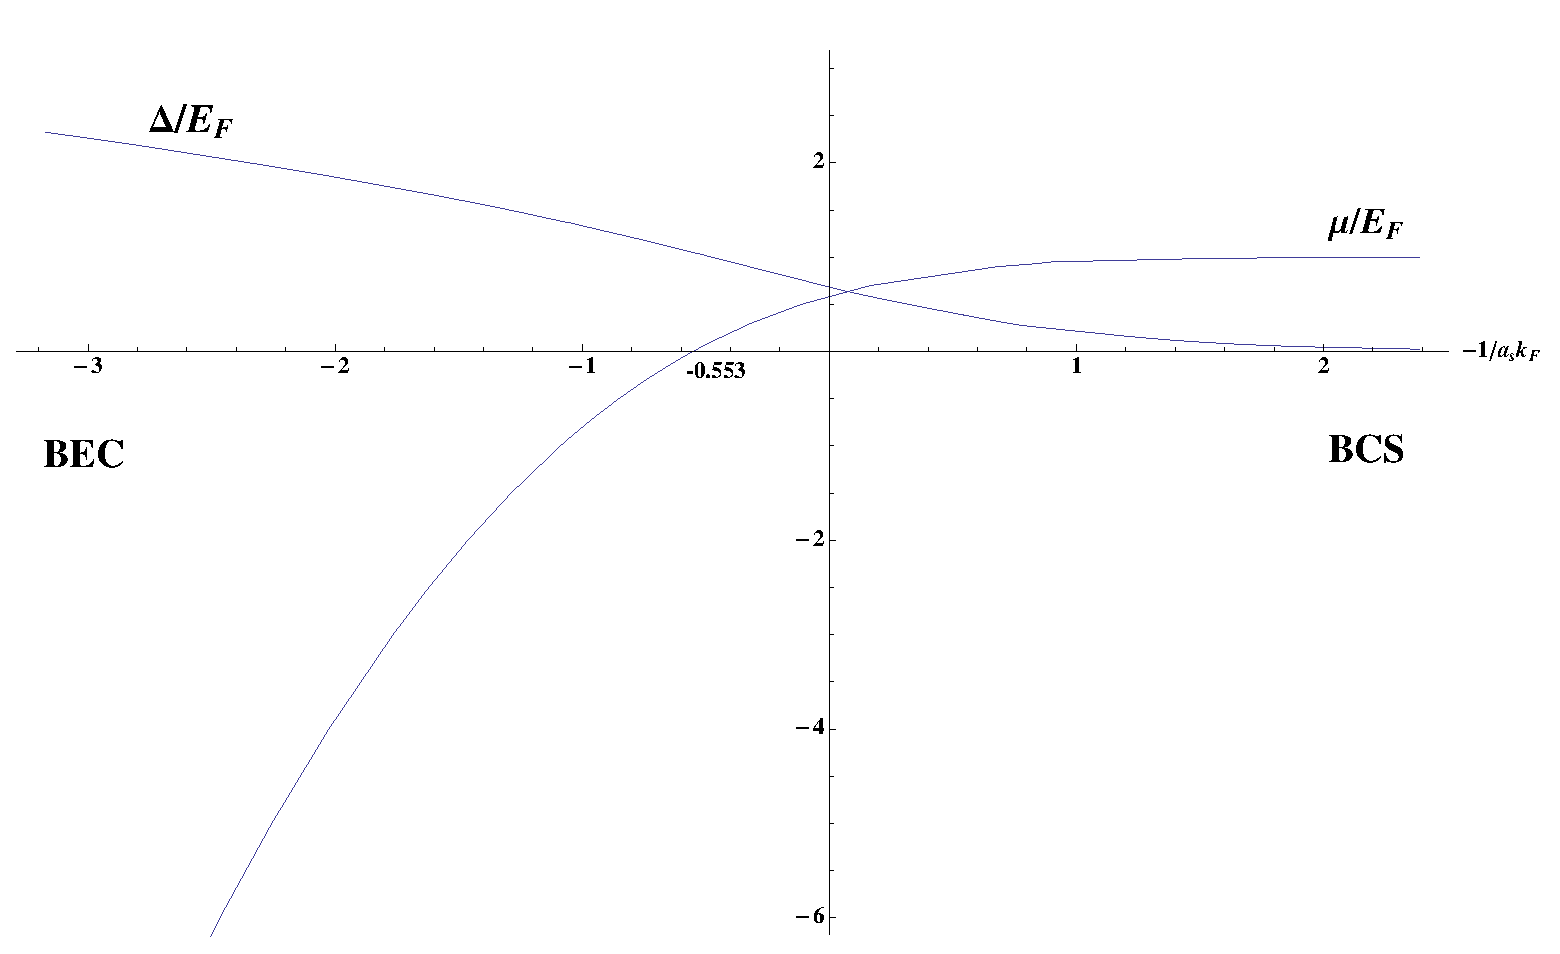
\includegraphics[width=0.8\textwidth]{SingleChannelCrossoverMuDelta}
\caption{The chemical potential $\mu$ and gap $\Delta$ in the mean field level over crossover} 
\label{fig:pathInt:meanField}
{\small All quantities in the unit of energy ($\mu$, $\Delta$) are rescaled with the Fermi energy $E_{F}$ and the s-wave scattering length $a_{s}$ is rescaled with $1/k_{F}$.  }
\end{center}
\end{figure}



\section{Gaussian fluctuation and collective modes}\label{sec:collective1}
We can expand the partition function Eq. (\ref{eq:pathInt:DeltaPF}) around the mean-field value, $\Delta(\vr,\tau)=\Delta_{0}+\theta(\vr,\tau)$. The linear order of the  expansion is zero because $\Delta_{0}$ is the saddle point.  The next order gives us the bilinear terms on $\theta$, i.e., correlation of bosonic fields $\Delta$ (four-fermion correlation).  Note that here the Hamiltonian only has a contact-type potential, therefore it cannot cover the situation of a charged system where long-range Columnb interaction cannot be neglected.  We limit ourselves to the neutual case.  Nevertheless, it is conceivable that a more realistic short-range potential only renormalizes some parameters in the following calculation while leaves the qualitative result unmodified.  

Notice that we can expand the second term in Eq. (\ref{eq:pathInt:DeltaPF}) for $\hat{G}{}^{-1}=\hat{G}_{0}^{-1}+\hat{K}$
\begin{equation}\label{eq:pathInt:expand}
\tr\ln \hat{G}^{-1}=\tr\ln\hat{G_{0}}^{-1}+\tr(\hat{G_{0}}\hat{K})-\nth{2}\tr(\hat{G_{0}}\hat{K}\hat{G_{0}}\hat{K})+\cdots
\end{equation}
In our case,
\begin{equation}
\hat{K}=\begin{pmatrix}
0&\theta\\
\theta^{*}&0
\end{pmatrix}
\end{equation}
Here the linear terms of $\hat{K}$ or $\theta$ ($\theta^{*}$) are zero as the saddle point condition.  To the second order, the action is 
\begin{equation}\label{eq:pathInt:DeltaActionGaussian}
S[\Delta_{0},\theta,\theta^{*}]=S[\Delta_{0}]+
	\nth{2g}\tr(\hat{K}\hat{K})+\nth{2}\tr(\hat{G_{0}}\hat{K}\hat{G_{0}}\hat{K})
\end{equation}
Write the last term into the momentum representation
\begin{equation}
\tr(\hat{G_{0}}\hat{K}\hat{G_{0}}\hat{K})=\sum_{q,p}\Tr\br{G_{0}({p})K_{q}G_{0}{}({p-q})K_{-q}}
\end{equation}
Notice that the second ``$\Tr$'' and following ``$\Tr$'' in this section only runs in Nambu spinor space and $q={(\vq,q_{l})}$, $p=(\vp,p_{n})$ are all four momentum, where $q_{l}$ is the bosonic Matsubara frequency while $p_{n}$ is the fermionic Matsubara frequency.
\begin{equation}
K_{p_{0},p_{0}+q}=K_{q}=\begin{pmatrix}
0&\theta_{q}\\
\theta^{*}_{-q}&0
\end{pmatrix}
\end{equation}
And we remember that $G_{0}(p)=G_{0}{}_{p,p}$
If we introduce  a new vector 
\begin{equation}
\theta{(q)}=\begin{pmatrix}\theta_{q}\\\theta^{*}_{-q}\end{pmatrix}\qquad
\theta^{\dg}{(q)}=\begin{pmatrix}\theta^{*}_{q}&\theta_{-q}\end{pmatrix}
\end{equation}
the action can be rewritten into a more compact form
\begin{equation}
S[\Delta_{0},\theta,\theta^{*}]=S[\Delta_{0}]+\nth{2}\sum_{q}\mbr{\theta^{\dg}(q)\mathbf{M}(q)\theta(q)}
\end{equation}
Notice that we can always choose a real $\Delta_{0}$ and therefore $G_{0}{\ _{12}}(p)=G_{0}{\ _{21}}(p)$, we have 
\begin{equation}
\mathbf{M}_{q,q}=\mathbf{M}(q)=
\begin{pmatrix}
\nth{g}+\sum_{p}G_{0}{\ }_{11}(p)G_{0}{\ }_{22}(p-q)&\sum_{p}G_{0}{\ }_{12}(p)G_{0}{\ }_{12}(p-q)\\
\sum_{p}G_{0}{\ }_{12}(p)G_{0}{\ }_{12}(p-q)&\nth{g}+\sum_{p}G_{0}{\ }_{11}(p-q)G_{0}{\ }_{22}(p)
\end{pmatrix}
\end{equation}
The summation over  the (fermionic) Matsubara frequency of $p_{n}$ can be carried out at zero temperature

\begin{equation}
\begin{split}
M_{11}(q)&=M_{22}(-q)\\
	&=\nth{g}+\sum_{\vp{,}p_{n}}G_{0}{\ }_{11}(p)G_{0}{\ }_{22}(p-q)\\
	&=\nth{g}+\sum_{\vp}\br{\frac{u^{2}u'^{2}}{iq_{l}-E-E'}-\frac{v^{2}v'^{2}}{iq_{l}+E+E'}}
\end{split}
\end{equation}
\begin{equation}
\begin{split}
M_{12}(q)&=M_{21}(q)\\
	&=\sum_{\vp{,}p_{n}}G_{0}{\ }_{12}(p)G_{0}{\ }_{12}(p-q)\\
	&=\sum_{\vp}uvu'v'\br{\nth{iq_{l}+E+E'}-\nth{iq_{l}-E-E'}}
\end{split}
\end{equation}
where $u=u_{\vp}$, $v=v_{\vp}$, $E=E_{\vp}$ and $u'=u_{\vp-\vq}$, $v'=v_{\vk-\vq}$, $E'=E_{\vk-\vq}$.  $u_{\vk}$, $v_{\vk}$, $E_{\vk}$ are as defined usually in BCS literature. 
\begin{equation}
v_{\vk}^{2}=1-u_{\vk}^{2}=\nth{2}\br{1-\frac{\xi_{\vk}}{E_{\vk}}}
\end{equation}
 The $G^{(M)}=\mathbf{M}^{-1}$ is the correlation function of $\theta$ (or $\Delta$) and its poles give the spectrum of collective modes as every  $\theta_{q}$ (or $\Delta_{q}$) involves many fermions moving in a coherent manner.  So the spectrum of collective modes can be determined by finding poles of $G^{(M)}$, $\det{M(\omega,\vq)}=0$ after we analytically continue for the frequency $iq_{l}\rightarrow\omega+i0^{+}$.  
 
For low energy modes, where $\omega,\,\abs{\vq}^{2}$ both are much smaller than $\min\bbr{E_{\vk}}=\Delta_{0}$ (or $\sqrt{\mu^{2}+\Delta^{2}}$ for $\mu<0$), we can expand $M$ with $\omega$ and $\vq$.  The lowest order has the form $\omega\approx{}c\,q$, which suggests a sound wave as expected for any Goldstone mode.  At BCS side, $c=v_{F}/\sqrt{3}$, where $v_{F}$ is Fermi velocity.  This coincides with the famous Anderson-Bogoliubov mode.  At the BEC side, we get $c^{2}=\Delta^{2}/8m\abs{\mu}=v_{F}^{2}(k_{F}a_{s})/3\pi=4\pi{}n_{B}a_{B}/m_{B}$, which fits the low momentum part of Bogoliubov spectrum of bosons gas.  Here $m_{B}=2m$ is the molecule mass, $n_{B}=n/2$ is the molecule density and $a_{B}=2a_{s}$ is the inferred  interaction between molecules.  This value differs from the result of more accurate calculation from the few-body theory, $a_{B}=0.6a_{s}$ \cite{Petrov}, which indicates the possible deficiency of the current theory. 


\section{An alternative method to invert the Green's function\label{sec:diagonalizeGreen1}}
In the above section, we inverted the  Gor'kov green function matrix Eqs. (\ref{eq:pathInt:nG}, \ref{eq:pathInt:G0}) directly and it is not hard to do as a $2\times2$ matrix in the  momentum space.   Alternatively, we can use a different approach which proves to be more convenient in the two-channel problem.  First, we diagonalize $\nG$ with a unitary transformation $T$, in the momentum space
\begin{equation}
\nG=\mtrx{i\omega_{n}-\xi_{k}&\Delta\\\bar\Delta&i\omega_{n}+\xi_{k}}=T^{\dg}BT
\end{equation}
It is easy to show that such $T$ and $B$ satisfying above equation are
\begin{equation}
T=\mtrx{u_{k}&v_{k}\\-v_{k}^{*}&u_{k}}\qquad{}B=\mtrx{i\omega_{n}+E_{k}&0\\0&i\omega_{n}-E_{k}}
\end{equation}
where $u_{k}^{2}(v_{k}^{2})=\nth{2}(1\pm\xi_{k}/E_{k})$ and $E_{k}=\sqrt{\xi^{2}_{\vk}+\Delta^{2}}$ are conventionally defined quantities in the BCS theory.   Actually, this transformation is nothing but the Bogoliubov canonical transformation, and the $B$ matrix simply describes the spectrum of the fermionic quasi-particles.  Now it is easy to invert $\nG$
\begin{equation}
\mathcal{G}=T^{\dg}B^{-1}T
\end{equation}
Green's function $\mathcal{G}$ takes a more conventional form $A/(i\omega_{n}\pm{}E_{k})$ without any dependency on frequency in nominator as Eq. (\ref{eq:pathInt:G0}). Matsubara frequency summation over $G_{0}(k)$ in the mean-field and $G_{0}(k)G_{0}(k+q)$ in the Gaussian order are then easier to perform  as in text-book.  




\begin{subappendices}
\end{subappendices}

